\documentclass[11pt]{article}
\usepackage[a4paper, margin=2cm]{geometry}
\usepackage{amsmath}
\usepackage{amssymb}
\usepackage{amsthm}
\usepackage{dsfont}
\usepackage{bbm}
\usepackage{multirow}
\usepackage{array}
\usepackage{diagbox}
\usepackage{makecell}
\newcolumntype{C}[1]{>{\centering\arraybackslash}m{#1}}
% \usepackage{charter}
\usepackage{fontspec}
% \usepackage{unicode-math}
\setmainfont{Charter}
% \setmathfont{XCharter-Math.otf}
% \usepackage{newtxtext,newtxmath}
\usepackage{braket}
\usepackage{slashed}
\usepackage{color}
\usepackage[table]{xcolor}
\usepackage[mathscr]{euscript}
\usepackage{graphicx}
\usepackage{placeins}
\usepackage{floatrow}
\floatsetup[table]{capposition=top}
\usepackage[caption=false]{subfig}
\usepackage[export]{adjustbox}
\floatsetup[figure]{style=plain,subcapbesideposition=top}
\usepackage{xfrac}
\usepackage{bm}
\usepackage{microtype}
\usepackage{commath}
\usepackage{mathtools}
\usepackage{enumitem}
\usepackage{xparse}
\usepackage[
    colorlinks=true, urlcolor=blue,
    linkcolor=blue, citecolor=blue
]{hyperref}% add hypertext capabilities
\usepackage{tikz}
\usepackage{ifthen}
\usepackage[framemethod=TikZ]{mdframed}
\usepackage[version=4]{mhchem}
\usepackage[numbers]{natbib}
\usepackage[nottoc]{tocbibind}
\usepackage[english]{babel}
\usepackage[autostyle, english = american]{csquotes}
\MakeOuterQuote{"}
\usepackage{setspace}

\usetikzlibrary{decorations.markings}
\usetikzlibrary{calc, positioning, arrows.meta}
\tikzset{midarrow/.style={
    decoration={markings, mark=at position 0.55 with {\arrow{>}}},
    postaction={decorate}
}}
\tikzset{midarrowrev/.style={
    decoration={markings, mark=at position 0.45 with {\arrow{<}}},
    postaction={decorate}
}}

% \allowdisplaybreaks

\theoremstyle{remark}
\newtheorem*{remark}{Remark}

\NewDocumentEnvironment{diagram}{O{0.68} O{0.75}}{
    \begin{tikzpicture}[
        baseline = (X.base),
        every node/.style={scale=#1}, scale=#2
    ]
}{\end{tikzpicture}}

\definecolor{green}{RGB}{50, 180, 50}
\definecolor{blue}{RGB}{20, 30, 250}

\newcommand{\pos}[2]{\begin{matrix}
    #1 \\ #2
\end{matrix}}
\newcommand{\dobase}[2]{
    \draw (#1,#2) node (X) {$\phantom{X}$};
}

\NewDocumentCommand{\lineH}{O{black} m m m}{
    \draw[color=#1] (#2,#4) -- (#3,#4);
}
\NewDocumentCommand{\lineHa}{O{black} m m m}{
    \draw[midarrow, color=#1] (#2,#4) -- (#3,#4);
}

\NewDocumentCommand{\lineV}{O{black} m m m}{
    \draw[color=#1] (#4,#2) -- (#4,#3);
}
\NewDocumentCommand{\lineVa}{O{black} m m m}{
    \draw[midarrow, color=#1] (#4,#2) -- (#4,#3);
}

\newcommand{\contrL}[3]{
    \draw (#3,#1) to[out=180,in=180] (#3,#2);
}
\newcommand{\contrLa}[3]{
    \draw[midarrow] (#3,#1) to[out=180,in=180] (#3,#2);
}

\newcommand{\contrR}[3]{
    \draw (#3,#1) to[out=0,in=0] (#3,#2);
}
\newcommand{\contrRa}[3]{
    \draw[midarrow] (#3,#1) to[out=0,in=0] (#3,#2);
}

\NewDocumentCommand{\rect}{m m m m m o}{
    \IfNoValueTF{#6}{
        \draw[rounded corners] 
        (#1 - #3/2, #2 - #4/2) 
        rectangle (#1 + #3/2, #2 + #4/2);
    }{
        \draw[rounded corners, fill=#6] 
        (#1 - #3/2, #2 - #4/2) 
        rectangle (#1 + #3/2, #2 + #4/2);
    }
    \node[align=center] at (#1,#2) {#5};
}

\newcommand{\tensor}[3]{
    \rect{#1}{#2}{1}{1}{#3}
}
\newcommand{\Tensora}[1]{
    \begin{diagram}
        \dobase{0}{0} \tensor{0}{0}{#1}
        \lineHa{-1}{-0.5}{0}
        \lineHa{0.5}{1}{0}
        \lineVa{-1}{-0.5}{0}
    \end{diagram}
}
\newcommand{\TensorAC}[1]{
    \begin{diagram}
        \dobase{0}{0} \tensor{0}{0}{#1}
        \lineHa{-1}{-0.5}{0}
        \lineHa{1}{0.5}{0}
        \lineVa{-1}{-0.5}{0}
    \end{diagram}
}

\newcommand{\tensorL}[3]{
    \draw (-0.5+#1,-0.5+#2) -- (0.25+#1,-0.5+#2) 
    -- (0.5+#1,0+#2) -- (0.25+#1,0.5+#2) 
    -- (-0.5+#1,0.5+#2) -- cycle;
    \draw (#1-0.07,#2) node {#3};
}
\newcommand{\TensorLa}[1]{
    \begin{diagram}
        \dobase{0}{0} \tensorL{0}{0}{#1}
        \lineHa{-1}{-0.5}{0}
        \lineHa{0.5}{1}{0}
        \lineVa{-1}{-0.5}{0}
    \end{diagram}
}

\newcommand{\tensorR}[3]{
    \draw (0.5+#1,-0.5+#2) -- (-0.25+#1,-0.5+#2) 
    -- (-0.5+#1,0+#2) -- (-0.25+#1,0.5+#2) 
    -- (0.5+#1,0.5+#2) -- cycle;
    \draw (#1+0.05,#2) node {#3};
}
\newcommand{\TensorRa}[1]{
    \begin{diagram}
        \dobase{0}{0} \tensorR{0}{0}{#1}
        \lineHa{-1}{-0.5}{0}
        \lineHa{0.5}{1}{0}
        \lineVa{-1}{-0.5}{0}
    \end{diagram}
}

\newcommand{\tensorU}[3]{
    \draw (-0.5+#1,0.5+#2) -- (0.5+#1,0.5+#2) 
    -- (0.5+#1,-0.25+#2) -- (0+#1,-0.5+#2) 
    -- (-0.5+#1,-0.25+#2) -- cycle;
    \draw (#1,#2+0.07) node {#3};
}
\newcommand{\tensorD}[3]{
    \draw (-0.5+#1,-0.5+#2) -- (0.5+#1,-0.5+#2) 
    -- (0.5+#1,0.25+#2) -- (0+#1,0.5+#2) 
    -- (-0.5+#1,0.25+#2) -- cycle;
    \draw (#1,#2-0.05) node {#3};
}

\newcommand{\fuserL}[5]{
    \draw (#1,#2-#3) -- (#1,#2+#3) 
    -- (#1-#4,#2) -- cycle;
    \node at (#1-0.4*#4,#2) {#5};
}
\newcommand{\fuserR}[5]{
    \draw (#1,#2-#3) -- (#1,#2+#3) 
    -- (#1+#4,#2) -- cycle;
    \node at (#1+0.4*#4,#2) {#5};
}

\NewDocumentCommand{\mat}{O{0.5} m m m}{
    \draw (#2,#3) circle (#1);
    \draw (#2,#3) node {#4};
}
\NewDocumentCommand{\Matrixa}{O{0.5} m}{
    \begin{diagram}
        \dobase{0}{0} \mat[#1]{0}{0}{#2}
        \lineHa{#1}{1}{0} \lineHa{-1}{-#1}{0}
    \end{diagram}
}
\NewDocumentCommand{\MatrixC}{O{0.5} m}{
    \begin{diagram}
        \dobase{0}{0} \mat[#1]{0}{0}{#2}
        \lineHa{1}{#1}{0} \lineHa{-1}{-#1}{0}
    \end{diagram}
}

\NewDocumentCommand{\weight}{O{0.5} m m m}
{\begin{scope}[shift={(#2,#3)}]
    \draw (-#1,0) -- (0,#1) -- (#1,0) -- (0,-#1) -- cycle;
    \node at (0,0) {#4};
\end{scope}}

\NewDocumentCommand{\bloba}{m m m m m}{
    % Get the parameters
    \def\xc{#1}
    \def\yc{#2}
    \def\inangles{#3}
    \def\outangles{#4}
    % Draw the circle at the specified coordinates
    \draw (\xc,\yc) circle (0.5);
    % Draw incoming arrows
    \foreach \angle in \inangles {
        \pgfmathsetmacro{\xstart}{\xc + 1.5*cos(\angle)}
        \pgfmathsetmacro{\ystart}{\yc + 1.5*sin(\angle)}
        \pgfmathsetmacro{\xend}{\xc + 0.5*cos(\angle)}
        \pgfmathsetmacro{\yend}{\yc + 0.5*sin(\angle)}
        \draw[midarrow] (\xstart, \ystart) -- (\xend, \yend);
    }
    % Draw outgoing arrows
    \foreach \angle in \outangles {
        \pgfmathsetmacro{\xstart}{\xc + 0.5*cos(\angle)}
        \pgfmathsetmacro{\ystart}{\yc + 0.5*sin(\angle)}
        \pgfmathsetmacro{\xend}{\xc + 1.5*cos(\angle)}
        \pgfmathsetmacro{\yend}{\yc + 1.5*sin(\angle)}
        \draw[midarrow] (\xstart, \ystart) -- (\xend, \yend);
    }
    \draw (#1,#2) node {#5};
}

\NewDocumentCommand{\blob}{m m m m}{
    % Get the parameters
    \def\xc{#1}
    \def\yc{#2}
    \def\angles{#3}
    % Draw the circle at the specified coordinates
    \draw (\xc,\yc) circle (0.5);
    % Draw incoming arrows
    \foreach \angle in \angles {
        \pgfmathsetmacro{\xstart}{\xc + 1.5*cos(\angle)}
        \pgfmathsetmacro{\ystart}{\yc + 1.5*sin(\angle)}
        \pgfmathsetmacro{\xend}{\xc + 0.5*cos(\angle)}
        \pgfmathsetmacro{\yend}{\yc + 0.5*sin(\angle)}
        \draw (\xstart, \ystart) -- (\xend, \yend);
    }
    \draw (#1,#2) node {#4};
}

\newcommand{\closeLeft}[2]
{\begin{scope}[shift={(#1,0)}]
    \draw (-1,0.5) to[out=90,in=180] (0,1.5);
    \draw (0,-1.5) to[out=180,in=270] (-1,-0.5);
    \mat{-1}{0}{#2}
\end{scope}}
\newcommand{\closeLefta}[2]
{\begin{scope}[shift={(#1,0)}]
    \draw[midarrow] (-1,0.5) to[out=90,in=180] (0,1.5);
    \draw[midarrow] (0,-1.5) to[out=180,in=270] (-1,-0.5);
    \mat{-1}{0}{#2}
\end{scope}}

\newcommand{\closeRight}[2]{
    \draw (#1,+1.5) to[out=0,in=90] (#1+1,0.5);
    \draw (#1+1,-0.5) to[out=270,in=0] (#1,-1.5);
    \mat{#1+1}{0}{#2}
}
\newcommand{\closeRighta}[2]{
    \draw[midarrow] (#1+1,0.5) to[out=90,in=0] (#1,+1.5);
    \draw[midarrow] (#1,-1.5) to[out=0,in=-90] (#1+1,-0.5);
    \mat{#1+1}{0}{#2}
}

\newcommand{\colmat}[3]{
    \tensor{#1}{1.5}{#2}
    \tensor{#1}{-1.5}{#3}
    \lineV{-1}{1}{#1}
}
\newcommand{\colmata}[3]{
    \tensor{#1}{1.5}{#2}
    \tensor{#1}{-1.5}{#3}
    \lineVa{-1}{1}{#1}
}

\newcommand{\colmatL}[3]{
    \tensorL{#1}{1.5}{#2}
    \tensorL{#1}{-1.5}{#3}
    \lineV{-1}{1}{#1}
}
\newcommand{\colmatLa}[3]{
    \tensorL{#1}{1.5}{#2}
    \tensorL{#1}{-1.5}{#3}
    \lineVa{-1}{1}{#1}
}

\newcommand{\colmatR}[3]{
    \tensorR{#1}{1.5}{#2}
    \tensorR{#1}{-1.5}{#3}
    \lineV{-1}{1}{#1}
}
\newcommand{\colmatRa}[3]{
    \tensorR{#1}{1.5}{#2}
    \tensorR{#1}{-1.5}{#3}
    \lineVa{-1}{1}{#1}
}

\newcommand{\applyTransferL}[3]{
    \begin{diagram}
        \dobase{0}{0}
        \colmat{0}{#1}{#3} \closeLeft{-0.5}{#2}
        \lineH{0.5}{1}{1.5} \lineH{0.5}{1}{-1.5}
    \end{diagram}
}
\newcommand{\applyTransferLa}[3]{
    \begin{diagram}
        \dobase{0}{0}
        \colmata{0}{#1}{#3} 
        \closeLefta{-0.5}{#2}
        \lineHa{0.5}{1}{1.5} 
        \lineHa{1}{0.5}{-1.5}
    \end{diagram}
}

\newcommand{\applyTransferR}[3]{
    \begin{diagram}
        \dobase{0}{0}
        \colmat{0}{#1}{#3} \closeRight{0.5}{#2}
        \lineH{-0.5}{-1}{1.5} \lineH{-0.5}{-1}{-1.5}
    \end{diagram}
}

\newcommand{\lrtimesMPS}[3]{
    \begin{diagram}
        \dobase{0}{0}
        \lineH{-3}{-2.5}{0}
        \mat{-2}{0}{#1}
        \lineH{-1.5}{-0.5}{0}
        \tensor{0}{0}{#2}
        \lineV{-1}{-0.5}{0}
        \lineH{0.5}{1.5}{0}
        \mat{2}{0}{#3}
        \lineH{2.5}{3}{0}
    \end{diagram}
}
\newcommand{\lrtimesMPSa}[3]{
    \begin{diagram}
        \dobase{0}{0}
        \lineHa{-3}{-2.5}{0}
        \mat{-2}{0}{#1}
        \lineHa{-1.5}{-0.5}{0}
        \tensor{0}{0}{#2}
        \lineVa{-1}{-0.5}{0}
        \lineHa{0.5}{1.5}{0}
        \mat{2}{0}{#3}
        \lineHa{2.5}{3}{0}
    \end{diagram}
}

\newcommand{\ltimesMPS}[2]{
    \begin{diagram}
        \dobase{0}{0}
        \mat{0}{0}{#1}
        \tensor{2}{0}{#2}
        \lineH{-1}{-0.5}{0}
        \lineH{0.5}{1.5}{0}
        \lineH{2.5}{3}{0}
        \lineV{-1}{-0.5}{2}
    \end{diagram}
}
\newcommand{\ltimesMPSa}[2]{
    \begin{diagram}
        \dobase{0}{0}
        \mat{0}{0}{#1}
        \tensor{2}{0}{#2}
        \lineHa{-1}{-0.5}{0}
        \lineHa{0.5}{1.5}{0}
        \lineHa{2.5}{3}{0}
        \lineVa{-1}{-0.5}{2}
    \end{diagram}
}

\newcommand{\rtimesMPS}[2]{
    \begin{diagram}
        \dobase{0}{0}
        \tensor{0}{0}{#1}
        \mat{2}{0}{#2}
        \lineH{-1}{-0.5}{0}
        \lineH{0.5}{1.5}{0}
        \lineH{2.5}{3}{0}
        \lineV{-1}{-0.5}{0}
    \end{diagram}
}
\newcommand{\rtimesMPSa}[2]{
    \begin{diagram}
        \dobase{0}{0}
        \tensor{0}{0}{#1}
        \mat{2}{0}{#2}
        \lineHa{-1}{-0.5}{0}
        \lineHa{0.5}{1.5}{0}
        \lineHa{2.5}{3}{0}
        \lineVa{-1}{-0.5}{0}
    \end{diagram}
}

% --------------------------------
% Special math fonts and notations
% --------------------------------

\newcommand{\graphics}[2]{\includegraphics[totalheight={#1}]{#2}}
\newcommand{\tr}{\operatorname{tr}}
\newcommand{\Abs}[1]{
    \left\lVert #1 \right\rVert
}
\newcommand{\bs}[1]{\boldsymbol{#1}}
\newcommand{\p}{\mathsf{P}}
\newcommand{\h}[1]{\ensuremath{\hat{#1}}}
\renewcommand{\t}[1]{\ensuremath{\tilde{#1}}}
\newcommand{\Z}{\ensuremath{\mathbb{Z}}}
\newcommand{\C}{\ensuremath{\mathbb{C}}}
\newcommand{\R}{\ensuremath{\mathbb{R}}}
\newcommand{\voperator}[1]{\ensuremath{\breve{#1}}}
\newcommand{\manifold}[1]{\ensuremath{\mathcal{#1}}}
\newcommand{\group}[1]{\ensuremath{\mathsf{#1}}}
\newcommand{\vectorspace}[1]{\ensuremath{\mathbb{#1}}}
\newcommand{\algebra}[1]{\ensuremath{\mathfrak{#1}}}
\newcommand{\pf}{\operatorname{pf}}

\newcommand{\Imag}{\mathrm{Im}}
\newcommand{\Real}{\mathrm{Re}}
\newcommand{\sgn}{\mathrm{sgn}}
\newcommand{\T}{\mathsf{T}}
\newcommand{\diag}{\mathrm{diag}}

\newcommand{\e}{\ensuremath{\mathrm{e}}}
\renewcommand{\d}{\ensuremath{\mathrm{d}}}
\renewcommand{\dag}{^\dagger}
\newcommand{\one}{\mathds{1}}
\newcommand{\ol}[1]{\overline{#1}}

\newcommand{\bA}{\bar{A}}
\newcommand{\tA}{\tilde{A}}
\newcommand{\bB}{\bar{B}}
\newcommand{\bG}{\bar{G}}
\newcommand{\tC}{\tilde{C}}

\newcommand{\vect}[1]{\ensuremath{\boldsymbol{#1}}}
\newcommand{\lv}{\ensuremath{\vect{v}_L^\dagger}}
\newcommand{\rv}{\ensuremath{\vect{v}_R}}
\newcommand{\spst}{\ensuremath{\ket{\{s\}}}}
\newcommand{\E}[2]{\ensuremath{E^{#1}_{#2}}}
\renewcommand{\O}[2]{\ensuremath{O^{#1}_{#2}}}
\renewcommand{\H}[4]{\ensuremath{H^{#1#2}_{#3#4}}}
\newcommand{\I}[6]{\ensuremath{I^{#1#2#3}_{#4#5#6}}}
\newcommand{\HH}[6]{\ensuremath{H^{#1#2#3}_{#4#5#6}}}
\newcommand{\J}[4]{\ensuremath{J^{#1#2}_{#3#4}}}
\newcommand{\alphap}{\ensuremath{{\alpha'}}}
\newcommand{\betap}{\ensuremath{{\beta'}}}
\newcommand{\gammap}{\ensuremath{{\gamma'}}}

% group theory
\newcommand{\U}{\ensuremath{\mathrm{U}}}
\newcommand{\SU}{\ensuremath{\mathrm{SU}}}
\newcommand{\su}{\ensuremath{\mathfrak{su}}}
\newcommand{\SO}{\ensuremath{\mathrm{SO}}}
\newcommand{\so}{\ensuremath{\mathfrak{so}}}

% category theory
\newcommand{\Hom}{\ensuremath{\mathrm{Hom}}}

\graphicspath{{./images/}}

\begin{document}

\section{VUMPS algorithm}

The \emph{variational uniform matrix product state (VUMPS)} algorithm \cite{VUMPS2018,Vanderstraeten2019,Nietner2020} is used to contract a 2D \emph{infinite uniform} tensor network at a relatively low computational cost. Unless otherwise stated, all tensors involved in the algorithm has even parity. 

\subsection{Uniform Matrix Product State}

An (infinite) \emph{uniform matrix product state} $\ket{\Psi}$ is an MPS that is invariant under translation by $N \ge 1$ sites. $\ket{\Psi}$ and its dual state $\bra{\Psi}$ are graphically represented by
\begin{equation}
    \ket{\Psi(A)} = \cdots
    \begin{diagram}
        \dobase{1.5}{0}
        \foreach \x in {0,2,4,6,8,10} {
            \lineHa{\x}{\x+1}{0}
        }
        \foreach \x in {1,3,5,7,9} {
            \lineVa{-1}{-0.5}{\x+0.5}
        }
        \tensor{1.5}{0}{$A_{n-2}$}
        \tensor{3.5}{0}{$A_{n-1}$}
        \tensor{5.5}{0}{$A_n$}
        \tensor{7.5}{0}{$A_{n+1}$}
        \tensor{9.5}{0}{$A_{n+2}$}
    \end{diagram} \cdots
\end{equation}
where $A_{n+N} = A_n$. The tensor $A^\dagger_n$ is the complex conjugate of $A_n$. Such a $\ket{\Psi(A)}$ is said to be in the \emph{uniform gauge}. Each tensor $A_n$ is only defined up to a gauge transformation
\begin{equation}
    \Tensora{$A_n$} \rightarrow 
    \lrtimesMPSa{$X^{-1}_{n-1}$}{$A_n$}{$X_n$}.
\end{equation}
where $X_{n+N} = X_n$. The dimensions of the physical and the virtual indices of tensors $A_n$ will be denoted as $D$ and $\chi$.

\subsection{Uniform MPS in Mixed Canonical Gauge}

The uniform MPS is usually put into the \emph{mixed canonical gauge} for easier contraction, which can be done in the following steps. 
\begingroup
\def\drawhlines{
    \lineHa{-1.5}{-0.5}{0}
    \lineHa{0.5}{1.5}{0}
    \lineHa{2.5}{3.5}{0}
}
\begin{itemize}
\item Use QR decomposition to iteratively solve the equations
\begin{equation}
    \begin{diagram}
        \dobase{0}{0} \drawhlines
        \mat{0}{0}{$L_{n-1}$}
        \tensor{2}{0}{$A_n$}
        \lineVa{-1}{-0.5}{2}
    \end{diagram} = \begin{diagram}
        \dobase{0}{0} \drawhlines
        \tensorL{0}{0}{$A^L_n$}
        \mat{2}{0}{$L_n$}
        \lineVa{-1}{-0.5}{0}
    \end{diagram}, \quad
    n = 1,2,...
\end{equation}
for the tensors $\{L_n\}$ and $\{A^L_n\}$. Since QR decomposition is unique (when diagonal elements of $R$ are required to be positive), the process will converge. 

\item Similarly, use LQ decomposition to iteratively solve the equations
\begin{equation}
    \begin{diagram}
        \dobase{0}{0} 
        \lineHa{-1.5}{-0.5}{0}
        \lineHa{0.5}{1.5}{0}
        \lineHa{3.5}{2.5}{0}
        \tensor{0}{0}{$A_n$}
        \mat{2}{0}{$R_{n+1}$}
        \lineVa{-1}{-0.5}{0}
    \end{diagram} = \begin{diagram}
        \dobase{0}{0} 
        \lineHa{-1.5}{-0.5}{0}
        \lineHa{1.5}{0.5}{0}
        \lineHa{3.5}{2.5}{0}
        \mat{0}{0}{$R_n$}
        \tensorR{2}{0}{$A^R_n$}
        \lineVa{-1}{-0.5}{2}
    \end{diagram}, \quad
    n = 1,2,...
\end{equation}
for the tensors $\{R_n\}$ and $\{A^R_n\}$. The choice of arrow directions on $R_n$ will reduce the amount of $P$ tensors needed in the algorithm. 

\item The tensors $\{A^L_n\}$ are left-unitary, and $\{A^R_n\}$ are right-unitary:
\begin{equation}
\begin{diagram}[0.7][0.7]
    \dobase{2.85}{0} \contrLa{-1.5}{1.5}{1}
    \colmatLa{1.5}{$A^L_n$}{$A^{L\dagger}_n$}
    \lineHa{2}{2.5}{1.5} 
    \lineHa{2.5}{2}{-1.5}
\end{diagram} = \begin{diagram}[0.7][0.7]
    \dobase{1.5}{0} \contrLa{-1.5}{1.5}{1}
\end{diagram}, \qquad
\begin{diagram}[0.7][0.7]
    \dobase{0}{0}
    \tensorR{0}{1.5}{$A^R_n$}
    \tensorR{0}{-1.5}{$A^{R\dagger}_n$}
    \lineHa{-0.5}{-1}{1.5}
    \lineHa{-1}{-0.5}{-1.5}
    \lineVa{-1}{1}{0}
    \contrRa{-1.5}{1.5}{0.5}
\end{diagram} = \begin{diagram}[0.7][0.7]
    \dobase{0}{0} \contrRa{-1.5}{1.5}{0}
\end{diagram}
\end{equation}

\item Gauge-transform the $\{A_n\}$ tensors using $\{L_n, R_n\}$ as
\begin{equation}
\begin{aligned}
    \begin{diagram}
        \dobase{0}{0}
        \tensorL{0}{0}{$A^L_n$}
        \lineHa{-1}{-0.5}{0}
        \lineHa{0.5}{1}{0}
        \lineVa{-1}{-0.5}{0}
    \end{diagram} &= \begin{diagram}
        \dobase{0}{0}
        \lineHa{-3}{-2.5}{0}
        \mat{-2}{0}{$L_{n-1}$}
        \lineHa{-1.5}{-0.5}{0}
        \tensor{0}{0}{$A_n$}
        \lineVa{-1}{-0.5}{0}
        \lineHa{0.5}{1.5}{0}
        \mat{2}{0}{$L^{-1}_n$}
        \lineHa{2.5}{3}{0}
    \end{diagram}
    \\
    \begin{diagram}
        \dobase{0}{0}
        \tensor{0}{0}{$A^C_n$}
        \lineHa{-1}{-0.5}{0}
        \lineHa{1}{0.5}{0}
        \lineVa{-1}{-0.5}{0}
    \end{diagram} &= \begin{diagram}
        \dobase{0}{0}
        \lineHa{-3}{-2.5}{0}
        \mat{-2}{0}{$L_{n-1}$}
        \lineHa{-1.5}{-0.5}{0}
        \tensor{0}{0}{$A_n$}
        \lineVa{-1}{-0.5}{0}
        \lineHa{0.5}{1.5}{0}
        \mat{2}{0}{$R_{n+1}$}
        \lineHa{3}{2.5}{0}
    \end{diagram}
    \\
    \begin{diagram}
        \dobase{0}{0}
        \tensorL{0}{0}{$A^R_n$}
        \lineHa{-0.5}{-1}{0}
        \lineHa{1}{0.5}{0}
        \lineVa{-1}{-0.5}{0}
    \end{diagram} &= \begin{diagram}
        \dobase{0}{0}
        \lineHa{-2.5}{-3}{0}
        \mat{-2}{0}{$R^{-1}_n$}
        \lineHa{-1.5}{-0.5}{0}
        \tensor{0}{0}{$A_n$}
        \lineVa{-1}{-0.5}{0}
        \lineHa{0.5}{1.5}{0}
        \mat{2}{0}{$R_{n+1}$}
        \lineHa{3}{2.5}{0}
    \end{diagram}
\end{aligned}
\label{eq:umps-canon-trans}
\end{equation}
where the inverse tensor $R^{-1}_n$ is defined from
\begin{equation}
\begin{diagram}
    \dobase{0}{0}
    \lineHa{-1.5}{-0.5}{0}
    \mat{0}{0}{$R_n$}
    \lineHa{1.5}{0.5}{0}
    \mat{2}{0}{$R^{-1}_n$}
    \lineHa{2.5}{3.5}{0}
\end{diagram} = \Matrixa{$I$}
\end{equation}
\end{itemize}
\endgroup
The \emph{mixed canonical gauge} is then ($\tr_v$ means contraction over all virtual indices):
\begin{align}
    & \ket{\Psi(A)}
    = \tr_v\Big[
        \cdots A_{n-2} A_{n-1} A_n 
        A_{n+1} A_{n+2} \cdots
    \Big]
    \nonumber \\
    &= \tr_v\Big[
        \cdots \underbrace{
            (L_{n-3} A_{n-2} L^{-1}_{n-2}) 
        }_{=A^L_{n-2}}
        \underbrace{
            (L_{n-2} A_{n-1} L^{-1}_{n-1}) 
        }_{=A^L_{n-1}}
        \underbrace{
            (L_{n-1} A_n R_{n+1}) 
        }_{=A^C_n}
        \underbrace{
            (R^{-1}_{n+1} A_{n+1} R_{n+2})
        }_{=A^R_{n+1}}
        \cdots
    \Big]
    \nonumber \\
    &= \cdots \begin{diagram}
        \dobase{1}{0}
        \foreach \x in {2,4,6,8,10} 
        {\lineVa{-1}{-0.5}{\x-0.5}}
        \foreach \x in {0,2,4} 
        {\lineHa{\x}{\x+1}{0}}
        \foreach \x in {6,8,10} 
        {\lineHa{\x+1}{\x}{0}}
        \tensorL{1.5}{0}{$A^L_{n-2}$} 
        \tensorL{3.5}{0}{$A^L_{n-1}$}
        \tensor{5.5}{0}{$A^C_n$}
        \tensorR{7.5}{0}{$A^R_{n+1}$} 
        \tensorR{9.5}{0}{$A^R_{n+2}$}
    \end{diagram}  \cdots
\end{align}
Introduce the matrix $C_n = L_n R_{n+1}$, which is related to the tensors $\{A^L_n, A^C_n, A^R_n\}$ by
\begin{equation}
    \TensorAC{$A^C_n$}
    = \begin{diagram}
        \dobase{0}{0} \lineVa{-1}{-0.5}{0}
        \tensorL{0}{0}{$A^L_n$}
        \mat{2}{0}{$C_n$}
        \lineHa{-1}{-0.5}{0}
        \lineHa{0.5}{1.5}{0}
        \lineHa{3}{2.5}{0}
    \end{diagram}
    = \begin{diagram}
        \dobase{0}{0} \lineVa{-1}{-0.5}{2}
        \mat{0}{0}{$C_{n-1}$}
        \tensorR{2}{0}{$A^R_n$}
        \lineHa{-1}{-0.5}{0}
        \lineHa{1.5}{0.5}{0}
        \lineHa{3}{2.5}{0}
    \end{diagram}
\end{equation}
Then the uniform MPS is put in the form
\begingroup
\newcommand{\drawlines}{
    \foreach \x in {0,2,4} 
    {\lineHa{\x}{\x+1}{0}}
    \foreach \x in {6,8,10} 
    {\lineHa{\x+1}{\x}{0}}
    \foreach \x in {1,3,7,9} 
    {\lineVa{-1}{-0.5}{\x+0.5}}
}
\begin{equation}
    \ket{\Psi(A)} 
    = \cdots \begin{diagram}
        \dobase{1.5}{0} \drawlines
        \tensorL{1.5}{0}{$A^L_{n-1}$} 
        \tensorL{3.5}{0}{$A^L_n$}
        \mat{5.5}{0}{$C_n$}
        \tensorR{7.5}{0}{$A^R_{n+1}$} 
        \tensorR{9.5}{0}{$A^R_{n+2}$}
    \end{diagram} \cdots
\end{equation}
\endgroup
Note that we still have the freedom to transform $\{A^L_n\}, \{A^R_n\}$ with a \emph{unitary} matrix without affecting the left and right unitary conditions:
\begin{align}
    A^L_i &\to U^\dagger_{i-1} A^L_i U_i
    \quad (i = \cdots, n-1, n) 
    \\
    A^R_j &\to V^\dagger_{j-1} A^R_j V_j
    \quad (j = n+1, n+2, \cdots)
\end{align}
To cancel the transformation of $A^L_n, A^R_n$, the center tensor $C$ should be changed to
\begin{equation}
    C_n \to U_n C_n V^\dagger_n
\end{equation}
Therefore, \emph{we can always make $C_n$ diagonal} by choosing $U_n, V_n$ obtained from the singular value decomposition of $C_n$. The singular values are actually the \emph{Schmidt weights} across the bond between $A^L_n$ and $A^R_{n+1}$ \cite{Mortier2024}. 

\subsubsection{Left and Right Canonical Gauges}

Alternatively, we can also convert the uniform MPS to the \emph{left canonical gauge} that only contains $\{A^L_n\}$ tensors
\begin{align}
    & \ket{\Psi(A)}
    = \tr_v\Big[
        \cdots \underbrace{
            (L_{n-2} A_{n-1} L^{-1}_{n-1}) 
        }_{=A^L_{n-1}}
        \underbrace{
            (L_{n-1} A_n L^{-1}_n) 
        }_{=A^L_n}
        \underbrace{
            (L_{n} A_{n+1} L^{-1}_{n+1}) 
        }_{=A^L_{n+1}} \cdots
    \Big]
    \nonumber \\
    &= \cdots \begin{diagram}
        \dobase{1}{0} \lineHa{0}{1}{0}
        \foreach \x in {2,4,6,8,10} {
            \lineHa{\x}{\x+1}{0}
            \lineVa{-1}{-0.5}{\x-0.5}
        }
        \tensorL{1.5}{0}{$A^L_{n-2}$} 
        \tensorL{3.5}{0}{$A^L_{n-1}$}
        \tensorL{5.5}{0}{$A^L_n$}
        \tensorL{7.5}{0}{$A^L_{n+1}$} 
        \tensorL{9.5}{0}{$A^L_{n+2}$}
    \end{diagram}  \cdots
\end{align}
or the \emph{right canonical gauge} that only contains $\{A^R_n\}$ tensors:
\begin{align}
    & \ket{\Psi(A)}
    = \tr_v\Big[
        \cdots \underbrace{
            (R^{-1}_{n-1} A_{n-1} R_n) 
        }_{=A^R_{n-1}}
        \underbrace{
            (R^{-1}_{n} A_{n} R_{n+1}) 
        }_{=A^R_n}
        \underbrace{
            (R^{-1}_{n+1} A_{n+1} R_{n+2}) 
        }_{=A^R_{n+1}} \cdots
    \Big]
    \nonumber \\
    &= \cdots \begin{diagram}
        \dobase{1}{0} \lineHa{1}{0}{0}
        \foreach \x in {2,4,6,8,10} {
            \lineHa{\x+1}{\x}{0}
            \lineVa{-1}{-0.5}{\x-0.5}
        }
        \tensorR{1.5}{0}{$A^R_{n-2}$} 
        \tensorR{3.5}{0}{$A^R_{n-1}$}
        \tensorR{5.5}{0}{$A^R_n$}
        \tensorR{7.5}{0}{$A^R_{n+1}$} 
        \tensorR{9.5}{0}{$A^R_{n+2}$}
    \end{diagram}  \cdots
\end{align}

\subsubsection{Solving \texorpdfstring{$A^L, A^R$}{AL, AR} from \texorpdfstring{$A^C, C$}{AC, C}}

Suppose that one only \emph{approximately} knows the center site tensors $\{A^C_n\}$ and $\{C_n\}$ of a uniform MPS. Naively, one may get $A^L, A^R$ from
\begin{equation*}
    A^L_n = A^C_n C^{-1}_n, \quad
    A^R_n = C^{-1}_{n-1} A^C_n
\end{equation*}
However, $A^L, A^R$ obtained in this way are not guaranteed to be unitary. Thus one actually obtains unitary $A^L, A^R$ by iteratively solving the optimization problems
\begin{equation}
    \min_{A^L_n} \Abs{A^C_n - A^L_n C_n}, \quad
    \min_{A^R_n} \Abs{A^C_n - C_{n-1} A^R_n}
\end{equation}
The solution is given by the left and right \emph{polar decompositions} of $A^C$ and $C$: 
\begin{gather}
    A^C_n = U^l_n P^l_n = P^r_n U^r_n,
    \quad
    C_n = U'^l_n P'^l_n = P'^r_n U'^r_n
    \\[0.2em] \Rightarrow \quad
    A^L_n = U^l_n (U'^l_n)^\dagger, \quad
    A^R_n = (U'^r_{n-1})^\dagger U^r_n
\end{gather}


\subsection{MPS Tangent Vectors}

Let $\mathbb{H}$ be the full Hilbert space of a system. The set of uniform MPS with physical dimension $D$ and virtual dimension $\chi$ can be regarded as a manifold $\mathcal{M}$ within $\mathbb{H}$. It is parametrized by the elements in tensors $A_1, ..., A_N$ ($N$ is the number of sites in a unit-cell); the parameter space is called $\mathbb{A}$, which has dimension $N D \chi^2$). 

\begin{figure}[t]
    \centering
    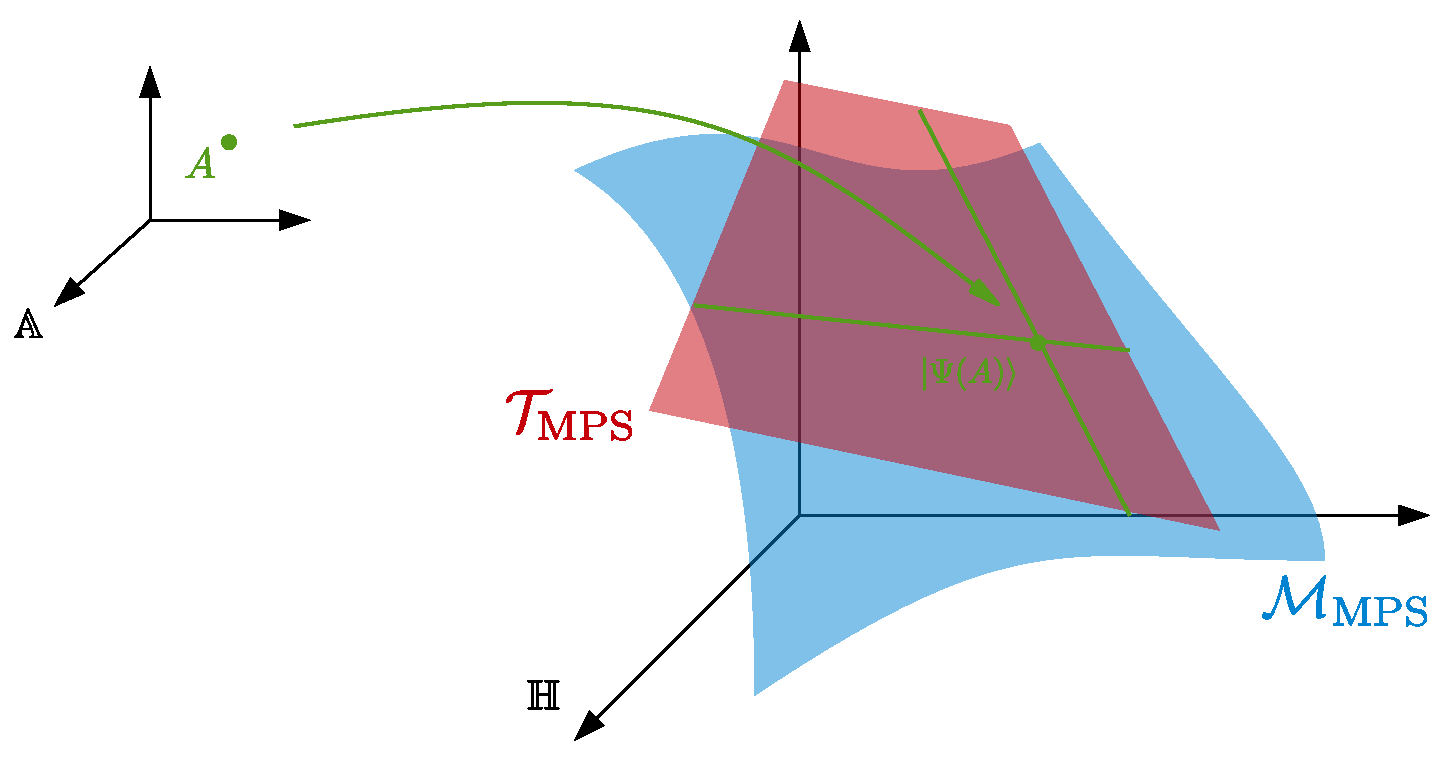
\includegraphics[scale=0.4]{tangent.pdf}
    \caption[
        The tangent space $\mathcal{T}_\text{MPS}$ at the MPS $\ket{\Psi(A)}$ on the MPS manifold $\mathcal{M}_\text{MPS}$. 
    ]{
        (Adapted from \cite{Vanderstraeten2019})
        The tangent space $\mathcal{T}_\text{MPS}$ at the MPS $\ket{\Psi(A)}$ on the MPS manifold $\mathcal{M}_\text{MPS}$. 
    }
\end{figure}

\subsubsection{Uniform Gauge}

At each uniform MPS $\ket{\Psi(A)} \in \mathcal{M}$, there is a \emph{tangent space} $\mathcal{T}_A \subset \mathbb{H}$ spanned by the derivatives with respect to elements of tensors $\{A_n\}$. In the uniform gauge, a tangent vector has the form
\begin{equation}
    \ket{\Phi(B;A)}
    = \sum_{n \in \Z} \cdots \begin{diagram}
        \dobase{0}{0} \lineHa{-6}{-5}{0}
        \foreach \x in {-4,-2,0,2,4} {
            \lineHa{\x}{\x+1}{0}
            \lineVa{-1}{-0.5}{\x-0.5}
        }
        \tensor{-4.5}{0}{$A_{n-2}$} 
        \tensor{-2.5}{0}{$A_{n-1}$} 
        \tensor{-0.5}{0}{$B_n$}
        \tensor{1.5}{0}{$A_{n+1}$}
        \tensor{3.5}{0}{$A_{n+2}$}
    \end{diagram} \cdots
\end{equation}
The tensor $B_n$ also has the periodicity $B_{n+N} = B_n$. 

\subsubsection{Gauge freedom of tangent MPS}

Similar to $\ket{\Psi(A)}$, the tangent vectors are also defined up to a gauge freedom. To show this, consider the following infinitesimal gauge transformation on $\ket{\Psi(A)}$:
\begin{equation}
\begin{aligned}
    A_n &\to e^{-\epsilon X_{n-1}} A_n e^{\epsilon X_n}
    = A_n + \epsilon G_n + O(\epsilon^2)
    \\
    G_n &\equiv A_n X_n - X_{n-1} A_n
    \quad (X_{n+N} = X_n)
\end{aligned}
\end{equation}
Thus $\ket{\Psi(A)}$ is changed to
\begin{equation}
    \ket{\Psi(A)} \to \ket{\Psi(A)}
    + \epsilon \ket{\Phi(G;A)} + O(\epsilon^2)
\end{equation}
But a gauge transformation actually does not change $\ket{\Psi(A)}$; therefore
\begin{equation}
    \forall \{X_n\}: \quad \ket{\Phi(G; A)} = 0
\end{equation}
As a result, any tangent vector $\ket{\Phi(B;A)}$ is \textit{invariant} under the change
\begin{equation}
    \Tensora{$B_n$} \rightarrow \Tensora{$B_n$} 
    + \rtimesMPSa{$A_n$}{$X_n$}
    - \ltimesMPSa{$X_{n-1}$}{$A_n$} 
\end{equation}
% Note that $\{B_n\}$ has $N D \chi^2$ parameters, while $\{X_n\}$ has $N \chi^2$ parameters. But $B_n$ is unchanged if all $X_n$ are the same and is proportional to the identity matrix. 

\subsubsection{Mixed Canonical Gauge}

Similar to Eq. \eqref{eq:umps-canon-trans}, if we define
\begin{equation}
    A^L_n = L_{n-1} A_n L^{-1}_n, \quad
    \tilde{B}_n = L_{n-1} B_n R_{n+1}, \quad
    A^R_n = R^{-1}_n A_n R_{n+1}
\end{equation}
then the tangent vector $\ket{\Phi(B;A)}$ can be converted to the mixed canonical form 
\begin{equation}
\ket{\Phi(\tilde{B};A^L,A^R)} 
= \sum_n \cdots\begin{diagram}
    \dobase{0}{0}
    \tensorL{-4.5}{0}{$A^L_{n-2}$} 
    \tensorL{-2.5}{0}{$A^L_{n-1}$} 
    \tensor{-0.5}{0}{$\tilde{B}_n$} 
    \tensorR{1.5}{0}{$A^R_{n+1}$} 
    \tensorR{3.5}{0}{$A^R_{n+2}$}
    % virtual
    \foreach \x in {-6,-4,-2} 
    {\lineHa{\x}{\x+1}{0}}
    \foreach \x in {0,2,4} 
    {\lineHa{\x+1}{\x}{0}}
    % physical
    \foreach \x in {-4,-2,0,2,4} 
    {\lineVa{-1}{-0.5}{\x-0.5}}
\end{diagram} \cdots
\end{equation}
The gauge freedom $B_n \to B_n + A_n X_n - X_{n-1} A_n$ in uniform gauge corresponds to the following gauge freedom in the mixed canonical gauge:
\begin{align}
    \tilde{B}_n &\to L_{n-1} (
        B_n + A_n X_n - X_{n-1} A_n
    ) R_{n+1}
    \nonumber \\
    &= \tilde{B}_n + A^L_n \tilde{X}_n
    - \tilde{X}_{n-1} A^R_n, 
\end{align}
where $\tilde{X}_n$ is defined as
\begin{equation}
    \MatrixC{$\tilde{X}_n$}
    = \begin{diagram}
        \dobase{0}{0}
        \lineHa{-3}{-2.5}{0}
        \mat{-2}{0}{$L_n$}
        \lineHa{-1.5}{-0.5}{0}
        \mat{0}{0}{$X_n$}
        \lineHa{0.5}{1.5}{0}
        \mat{2}{0}{$R_{n+1}$}
        \lineHa{3}{2.5}{0}
    \end{diagram}. 
\end{equation}
We often impose the \emph{left gauge-fixing condition} on $\{\tilde{B}_n\}$:
\begingroup
\newcommand{\drawlines}{
    \contrLa{-1}{1}{-0.5}
    \lineVa{-0.5}{0.5}{0}
    \lineHa{0.5}{1}{1} \lineHa{1}{0.5}{-1}
}
\begin{equation}
0 = \begin{diagram}[0.7][0.7]
    \dobase{0}{0} \drawlines
    \tensor{0}{1}{$\tilde{B}_n$}
    \tensorL{0}{-1}{$A^{L\dagger}_n$}
\end{diagram} = \begin{diagram}[0.7][0.7]
    \dobase{0}{0} \drawlines
    \tensorL{0}{1}{$A^L_n$}
    \tensor{0}{-1}{$\tilde{B}^\dagger_n$}
\end{diagram}
\label{eq:left-gauge-fix}
\end{equation}
\endgroup
The second equality is obtained by a Hermitian conjugate. The condition is only applicable to the tangent vectors that are orthogonal to $\ket{\Psi(A)}$, since it implies that
\begin{equation}
    \braket{\Psi(A)|\Phi(B;A)}
    = \sum_n \begin{diagram}
        \dobase{0}{0}
        \tensor{0}{1}{$\tilde{B}_n$}
        \tensor{0}{-1}{$A^{C\dagger}_n$}
        \lineVa{-0.5}{0.5}{0}
        \contrLa{-1}{1}{-0.5}
        \contrRa{-1}{1}{0.5}
    \end{diagram}
    = \sum_n \begin{diagram}
        \dobase{0}{0}
        \lineHa{2}{0.5}{1}
        \tensor{0}{1}{$\tilde{B}_n$}
        \tensorL{0}{-1}{$A^{L\dagger}_n$}
        \lineHa{1}{0.5}{-1}
        \tensor{1.5}{-1}{$C^\dagger_n$}
        \lineVa{-0.5}{0.5}{0}
        \contrLa{-1}{1}{-0.5}
        \contrRa{-1}{1}{2}
    \end{diagram}
    = 0
\end{equation}
From now on we drop the tilde on $B, X$ in the mixed canonical form. 

\subsubsection{Effective Parametrization}

\begingroup
Non-redundant parameters of the tangent space can be extracted to a matrix $X_n$ by QR decomposition:
\newcommand{\drawlines}{
    \contrLa{-1}{1}{-0.5}
    \lineVa{-0.5}{0.5}{0}
    \lineHa{1}{0.5}{-1}
}
\begin{equation}
    \TensorAC{$B_n$} = \begin{diagram}
        \dobase{0}{0} \lineVa{-1}{-0.5}{0}
        \tensorL{0}{0}{$V^L_n$}
        \mat{2}{0}{$X_n$}
        \lineHa{-1}{-0.5}{0}
        \lineHa{0.5}{1.5}{0}
        \lineHa{3}{2.5}{0}
    \end{diagram}
    \quad \text{where} \quad
    \begin{diagram}
        \dobase{0}{0} \drawlines
        \lineHa{0.5}{1}{1}
        \tensorL{0}{1}{$V^L_n$}
        \tensorL{0}{-1}{$V^{L\dagger}_n$}
    \end{diagram} = \begin{diagram}
        \dobase{1}{0}
        \contrLa{-1}{1}{1}
    \end{diagram}
\end{equation}
Then the left gauge-fixing condition Eq. \eqref{eq:left-gauge-fix} on $B$ implies
\begin{equation}
    0 = \begin{diagram}
        \dobase{0}{0} \drawlines
        \lineHa{1}{0.5}{1}
        \tensor{0}{1}{$B_n$}
        \tensorL{0}{-1}{$A^{L\dagger}_n$}
    \end{diagram}
    = \begin{diagram}
        \dobase{1}{0} \drawlines
        \lineHa{0.5}{1}{1}
        \tensorL{0}{1}{$V^L_n$}
        \mat{1.5}{1}{$X_n$}
        \lineHa{2.5}{2}{1}
        \tensorL{0}{-1}{$A^{L\dagger}_n$}
        \lineH{1}{2.5}{-1}
    \end{diagram}
    \quad \Rightarrow \quad
    \begin{diagram}
        \dobase{1}{0} \drawlines
        \lineHa{0.5}{1}{1}
        \tensorL{0}{1}{$V^L_n$}
        \tensorL{0}{-1}{$A^{L\dagger}_n$}
    \end{diagram} =  0
\end{equation}
\endgroup
Tensors $\{V^L_n\}$ can be further proved to satisfy
\begingroup
\newcommand{\drawlines}{
    \contrRa{-0.5}{1.5}{2}
    \lineHa{1}{0.5}{1.5}
    \lineHa{0.5}{1}{-0.5}
    \lineVa{2}{2.5}{1.5}
    \lineVa{-1.5}{-1}{1.5}
}
\begin{equation}
    \begin{diagram}
        \dobase{1}{0.5}
        \drawlines
        \tensorL{1.5}{1.5}{$V^{L\dagger}_n$}
        \tensorL{1.5}{-0.5}{$V^L_n$}
    \end{diagram} \quad = \quad \begin{diagram}
        \dobase{1}{0.5}
        \contrRa{-0.5}{1.5}{0.5}
        \lineVa{-1.5}{2.5}{2}
    \end{diagram} \quad - \quad \begin{diagram}
        \dobase{1}{0.5}
        \drawlines
        \tensorL{1.5}{1.5}{$A^{L\dagger}_n$}
        \tensorL{1.5}{-0.5}{$A^L_n$}
    \end{diagram}
    \label{eq:VLn-complement}
\end{equation}
\endgroup
The norm of two tangent vector $\braket{\Phi(B';A^L,A^R)|\Phi(B;A^L,A^R)}$ can be greatly simplified by the unitary conditions of $A^L, A^R$ and the left gauge-fixing  
\begin{equation}
    \braket{\Phi(B';A^L,A^R)|\Phi(B;A^L,A^R)}
    = \sum_{n \in \Z} \begin{diagram}
        \dobase{0}{0} \lineVa{-0.5}{0.5}{0}
        \contrLa{-1}{1}{-0.5} 
        \contrRa{-1}{1}{0.5}
        \tensor{0}{1}{$B_n$} 
        \tensor{0}{-1}{$B'^\dagger_n$} 
    \end{diagram}
    = \sum_{n \in \Z} \begin{diagram}
        \dobase{0}{0} 
        \contrLa{-1}{1}{-0.5} 
        \contrRa{-1}{1}{0.5}
        \mat{0}{1}{$X_n$} 
        \mat{0}{-1}{$X'^\dagger_n$} 
    \end{diagram},
\end{equation}
which is just the Euclidean inner product in the effective parameter space. 

\subsection{Projection to the Tangent Space}

Let $\ket{\Phi(B(X);A^L,A^R)}$ be the projection of a vector $\ket{\chi} \in \mathbb{H}$ on the tangent space at $\ket{\Psi(A)}$. Let $\mathcal{P}_A$ be the projection operator to the tangent space $\mathcal{T}_A$ at $\ket{\Psi(A)}$:
\begin{equation}
    \ket{\Phi(B(X);A^L,A^R)} 
    = \mathcal{P}_A \ket{\chi}.
\end{equation}
The parameter matrix $X$ of the tangent vector is the solution of the minimization problem
\begin{align*}
    & \min_X \Abs{
        \ket{\chi} - \ket{\Phi(B(X);A^L,A^R)}
    }^2
    \\
    &= \min_X \Big[
        \braket{\chi|\chi}
        + \underbrace{
            \braket{\Phi(B(X);A^L,A^R)|\Phi(B(X);A^L,A^R)}
        }_{= \sum_n \tr(X_n X^\dagger_n)}
        \\ &\quad
        - \braket{\chi|\Phi(B(X);A^L,A^R)}
        - \braket{\Phi(B(X);A^L,A^R)|\chi}
    \Big].
\end{align*}
The target function is quadratic in $\{X_n\}$ and $\{\bar{X}_n\}$. Therefore, 
\begin{equation}
    \frac{\partial}{\partial \bar{X}_n}
    \Abs{
        \ket{\chi} - \ket{\Phi(B(X);A^L,A^R)}
    }^2 = 0
    \ \Rightarrow \ 
    N_c X_n = \frac{\partial}{\partial \bar{X}_n}
    \braket{\Phi(B(X);A^L,A^R)|\chi},
\end{equation}
where $N_c \to \infty$ is the size (number of unit-cells) of the system. Graphically, the derivative removes tensor $\bar{X}$ from $\bra{\Phi(B(X);A^L,A^R)}$, and the factor $N_c$ can be removed by a proper normalization of $\ket{\chi}$:
\begin{equation}
    \MatrixC{$X_n$} = \begin{diagram}
        \dobase{0}{1.5}
        \node at (-0.5,1.5) {$\cdots$};
        \node at (12.5,1.5) {$\cdots$};
        \node at (-0.5,0) {$\cdots$};
        \node at (12.5,0) {$\cdots$};
        \contrRa{-1.5}{0}{6} 
        \contrLa{-1.5}{0}{8}
        \lineHa{5}{6}{-1.5} 
        \lineHa{9}{8}{-1.5}
        \lineH{0}{12}{1}
        \lineH{0}{12}{2}
        \draw (6,1.5) node {$\chi$};
        % virtual indices
        \foreach \x in {0,2,4} 
        {\lineHa{\x+1}{\x}{0}}
        \foreach \x in {9,11} 
        {\lineHa{\x}{\x+1}{0}}
        % physical indices
        \foreach \x in {1,3,5,8,10} {
            \lineVa{0.5}{1}{\x+0.5}
        }
        \tensorL{1.5}{0}{$A^{L\dagger}_{n-2}$}
        \tensorL{3.5}{0}{$A^{L\dagger}_{n-1}$}
        \tensorL{5.5}{0}{$V^{L\dagger}_n$}
        \tensorR{8.5}{0}{$A^{R\dagger}_{n+1}$}
        \tensorR{10.5}{0}{$A^{R\dagger}_{n+2}$}
    \end{diagram}
\end{equation}
Then the full tangent vector $\ket{\Phi(B(X);A^L,A^R)}$ is 
\begingroup
\def\drawproj{
    \node at (-0.5,1) {$\cdots$};
    \node at (12.5,1) {$\cdots$};
    \node at (-0.5,-1) {$\cdots$};
    \node at (12.5,-1) {$\cdots$};
    % virtual indices
    \foreach \x in {0,2,4} {
        \lineHa{\x+1}{\x}{1}
        \lineHa{\x}{\x+1}{-1}
    }
    \foreach \x in {9,11} {
        \lineHa{\x}{\x+1}{1}
        \lineHa{\x+1}{\x}{-1}
    }
    % physical indices
    \foreach \x in {1,3,5,8,10} {
        \lineVa{1.5}{2}{\x+0.5}
        \lineVa{-2}{-1.5}{\x+0.5}
    }
    \tensorL{1.5}{1}{$A^{L\dagger}_{n-2}$}
    \tensorL{3.5}{1}{$A^{L\dagger}_{n-1}$}
    \tensorL{5.5}{1}{$V^{L\dagger}_n$}
    \tensorR{8.5}{1}{$A^{R\dagger}_{n+1}$}
    \tensorR{10.5}{1}{$A^{R\dagger}_{n+2}$}
    \tensorL{1.5}{-1}{$A^L_{n-2}$}
    \tensorL{3.5}{-1}{$A^L_{n-1}$}
    \tensorL{5.5}{-1}{$V^L_n$}
    \tensorR{8.5}{-1}{$A^R_{n+1}$}
    \tensorR{10.5}{-1}{$A^R_{n+2}$}
    \contrRa{-1}{1}{6}
    \contrLa{1}{-1}{8}
}
\begin{equation}
    \ket{\Phi(B(X);A^L,A^R)} 
    = \sum_n \begin{diagram}
        \dobase{6}{2.5}
        \lineH{0}{12}{2}
        \lineH{0}{12}{3}
        \node at (-0.5,2.5) {$\cdots$};
        \node at (12.5,2.5) {$\cdots$};
        \draw (6,2.5) node {$\chi$};
        \drawproj
    \end{diagram} 
\end{equation}
Therefore, the projector $\mathcal{P}_A$ is
\begin{equation}
    \mathcal{P}_A = \sum_n
    \begin{diagram}
        \dobase{6}{0}
        \drawproj
    \end{diagram}
\end{equation}
which can also be rewritten using Eq. \eqref{eq:VLn-complement} as
\begin{equation}
\begin{aligned}
    \mathcal{P}_A = & \sum_n \begin{diagram}
        \dobase{1.5}{0}
        \tensorL{1.5}{1}{$A^{L\dagger}_{n-2}$}
        \tensorL{3.5}{1}{$A^{L\dagger}_{n-1}$}
        \tensorR{7.5}{1}{$A^{R\dagger}_{n+1}$}
        \tensorR{9.5}{1}{$A^{R\dagger}_{n+2}$}
        \tensorL{1.5}{-1}{$A^L_{n-2}$}
        \tensorL{3.5}{-1}{$A^L_{n-1}$}
        \tensorR{7.5}{-1}{$A^R_{n+1}$}
        \tensorR{9.5}{-1}{$A^R_{n+2}$}
        % virtual indices
        \foreach \x in {0,2} {
            \lineHa{\x+1}{\x}{1}
            \lineHa{\x}{\x+1}{-1}
        }
        \foreach \x in {8,10} {
            \lineHa{\x}{\x+1}{1}
            \lineHa{\x+1}{\x}{-1}
        }
        % physical indices
        \foreach \x in {1,3,5,7,9} {
            \lineVa{1.5}{2}{\x+0.5}
            \lineVa{-2}{-1.5}{\x+0.5}
        }
        \lineV{-1.5}{1.5}{5.5}
        \contrRa{-1}{1}{4}
        \contrLa{1}{-1}{7}
        \node at (-0.5,1) {$\cdots$};
        \node at (11.5,1) {$\cdots$};
        \node at (-0.5,-1) {$\cdots$};
        \node at (11.5,-1) {$\cdots$};
    \end{diagram}
    \\[1em] 
    - & \sum_n \begin{diagram}
        \dobase{1.5}{0}
        \tensorL{1.5}{1}{$A^{L\dagger}_{n-2}$}
        \tensorL{3.5}{1}{$A^{L\dagger}_{n-1}$}
        \tensorL{5.5}{1}{$A^{L\dagger}_n$}
        \tensorR{8.5}{1}{$A^{R\dagger}_{n+1}$}
        \tensorR{10.5}{1}{$A^{R\dagger}_{n+2}$}
        \tensorL{1.5}{-1}{$A^L_{n-2}$}
        \tensorL{3.5}{-1}{$A^L_{n-1}$}
        \tensorL{5.5}{-1}{$A^L_n$}
        \tensorR{8.5}{-1}{$A^R_{n+1}$}
        \tensorR{10.5}{-1}{$A^R_{n+2}$}
        % virtual indices
        \foreach \x in {0,2,4} {
            \lineHa{\x+1}{\x}{1}
            \lineHa{\x}{\x+1}{-1}
        }
        \foreach \x in {9,11} {
            \lineHa{\x}{\x+1}{1}
            \lineHa{\x+1}{\x}{-1}
        }
        % physical indices
        \foreach \x in {1,3,5,8,10} {
            \lineVa{1.5}{2}{\x+0.5}
            \lineVa{-2}{-1.5}{\x+0.5}
        }
        \contrRa{-1}{1}{6}
        \contrLa{-1}{1}{8}
        \node at (-0.5,1) {$\cdots$};
        \node at (12.5,1) {$\cdots$};
        \node at (-0.5,-1) {$\cdots$};
        \node at (12.5,-1) {$\cdots$};
    \end{diagram}
\end{aligned}
\end{equation}
\endgroup

\subsection{Optimization of Overlap}

Given a uniform MPS $\ket{\Psi(\tilde{A})}$, suppose we want to approximate it with another uniform MPS $\ket{\Psi(A)}$ with a different (usually smaller) bond dimension, such that their (normalized) overlap is maximized, i.e.
\begin{equation}
    \max_A \frac{
        |\braket{\Psi(A)|\Psi(\tilde{A})}|^2
    }{
        \braket{\Psi(A)|\Psi(A)}
    }
\end{equation}
For the optimal solution of $\ket{\Psi(A)}$, the projection of $\ket{\Psi(\tilde{A})}$ to the tangent space $\mathcal{T}_A$ is 0, i.e.
\begin{align*}
    0 &= \mathcal{P}_A \ket{\Psi(\tilde{A})} 
    \\
    &\equiv \sum_n \cdots \begin{diagram}
        \dobase{0}{0} 
        \tensorL{-4.5}{0}{$A^L_{n-2}$} 
        \tensorL{-2.5}{0}{$A^L_{n-1}$} 
        \tensor{-0.5}{0}{$G_n$} 
        \tensorR{1.5}{0}{$A^R_{n+1}$} 
        \tensorR{3.5}{0}{$A^R_{n+2}$}
        % virtual
        \foreach \x in {-6,-4,-2} 
        {\lineHa{\x}{\x+1}{0}}
        \foreach \x in {0,2,4} 
        {\lineHa{\x+1}{\x}{0}}
        % physical
        \foreach \x in {-4,-2,0,2,4} 
        {\lineVa{-1}{-0.5}{\x-0.5}}
    \end{diagram} \cdots
    = \ket{\Phi(G;A^L,A^R)}.
\end{align*}
The tensors $\{G_n\}$ in the tangent vector should be 0:
\begin{equation}
    G_n = A'^C_n - A^L_n C'_n \overset{!}{=} 0, 
\end{equation}
where $\{A'^C_n\}$ and $\{C'_n\}$ are given by
\begingroup
\newcommand{\drawlines}{
    \foreach \x in {0,2,4} {
        \lineHa{\x}{\x+1}{1}
        \lineHa{\x+1}{\x}{-1}
    }
    \foreach \x in {6,8,10} {
        \lineHa{\x+1}{\x}{1}
        \lineHa{\x}{\x+1}{-1}
    }
    \lineHa{4.5}{5}{-2}
    \lineHa{6.5}{6}{-2}
    \foreach \x in {1,3,7,9} {
        \lineVa{-0.5}{0.5}{\x+0.5}
    }
    \contrRa{-2}{-1}{5}
    \contrLa{-2}{-1}{6}
    \node at (-0.5,1) {$\cdots$};
    \node at (11.5,1) {$\cdots$};
    \node at (-0.5,-1) {$\cdots$};
    \node at (11.5,-1) {$\cdots$};
}
\begin{align}
    \TensorAC{$A'^C_n$} &= \begin{diagram}
        \dobase{5}{0}
        \drawlines
        \tensorL{1.5}{1}{$\tilde{A}^L_{n-2}$}
        \tensorL{3.5}{1}{$\tilde{A}^L_{n-1}$}
        \tensor{5.5}{1}{$\tilde{A}^C_n$}
        \tensorR{7.5}{1}{$\tilde{A}^R_{n+1}$}
        \tensorR{9.5}{1}{$\tilde{A}^R_{n+2}$}
        \tensorL{1.5}{-1}{$A^{L\dagger}_{n-2}$}
        \tensorL{3.5}{-1}{$A^{L\dagger}_{n-1}$}
        \tensorR{7.5}{-1}{$A^{R\dagger}_{n+1}$}
        \tensorR{9.5}{-1}{$A^{R\dagger}_{n+1}$}
        \lineVa{-2.5}{0.5}{5.5}
    \end{diagram}
    \label{eq:updateAC}
    \\
    \MatrixC{$C'_n$} &= \begin{diagram}
        \dobase{5}{0}
        \drawlines
        \tensorL{1.5}{1}{$\tilde{A}^L_{n-1}$}
        \tensorL{3.5}{1}{$\tilde{A}^L_n$}
        \mat{5.5}{1}{$\tilde{C}_n$}
        \tensorR{7.5}{1}{$\tilde{A}^R_{n+1}$}
        \tensorR{9.5}{1}{$\tilde{A}^R_{n+2}$}
        \tensorL{1.5}{-1}{$A^{L\dagger}_{n-1}$}
        \tensorL{3.5}{-1}{$A^{L\dagger}_n$}
        \tensorR{7.5}{-1}{$A^{R\dagger}_{n+1}$}
        \tensorR{9.5}{-1}{$A^{R\dagger}_{n+1}$}
    \end{diagram}
    \label{eq:updateC}
\end{align}
\endgroup
In $C'_n$, we have replaced $\tilde{A}^C_n$ by $\tilde{A}^L_n \tilde{C}_n$. Therefore, the optimal $\ket{\Psi(A)}$ can be solved from the equations
\begin{equation}
    A^L_n C_n = C_{n-1} A^R_n = A^C_n, \quad
    A^C_n = A^L_n C_n.
\end{equation}
iteratively as follows:
\begin{enumerate}
    \item Start from random or guessed tensors $\{A^L_n\}$, $\{A^C_n\}$, $\{A^R_n\}$, $\{C_n\}$ of $\ket{\Psi(A)}$. 
    
    \item Solve for the left fixed points $\{F^L_n\}$ ($F^L_{n+N} = F^L_n$) defined from
    \newcommand{\drawFL}[1]{
        \closeLefta{-0.5}{$F^L_{#1}$}
    }
    \begin{equation}
        \begin{diagram}
            \dobase{0}{0} \drawFL{n}
            \colmatLa{0}{$\tilde{A}^L_{n+1}$}{$A^{L\dagger}_{n+1}$}
            \lineHa{0.5}{1}{1.5}
            \lineHa{1}{0.5}{-1.5}
            \draw (1.5,1.5) node {$\cdots$};
            \draw (1.5,-1.5) node {$\cdots$};
            \lineHa{2}{2.5}{1.5}
            \lineHa{2.5}{2}{-1.5}
            \colmatLa{3}{$\tilde{A}^L_{n+N}$}{$A^{L\dagger}_{n+N}$}
            \lineHa{3.5}{4}{1.5}
            \lineHa{4}{3.5}{-1.5}
        \end{diagram} = \begin{diagram}
            \dobase{-1}{0} \drawFL{n}
        \end{diagram}
        \quad \Leftrightarrow \quad 
        \begin{diagram}
            \dobase{-1}{0} \drawFL{n-1}
            \colmatLa{0}{$\tilde{A}^L_n$}{$A^{L\dagger}_n$}
            \lineHa{1}{0.5}{1.5}
            \lineHa{0.5}{1}{-1.5}
        \end{diagram}
        = \begin{diagram}
            \dobase{-1}{0} \drawFL{n}
        \end{diagram}
    \end{equation}

    \item Solve for the right fixed points $\{F^R_n\}$ ($F^R_{n+N} = F^R_n$) defined from
    \newcommand{\drawFR}[1]{
        \closeRighta{0.5}{$F^R_{#1}$}
    }
    \begin{equation}
        \begin{diagram}
            \dobase{0}{0} \drawFR{n+1}
            \lineHa{-0.5}{-1}{1.5}
            \lineHa{-1}{-0.5}{-1.5}
            \colmatRa{0}{$\tilde{A}^R_{n+N}$}{$A^{R\dagger}_{n+N}$}
            \draw (-1.5,1.5) node {$\cdots$};
            \draw (-1.5,-1.5) node {$\cdots$};
            \lineHa{-2}{-2.5}{1.5}
            \lineHa{-2.5}{-2}{-1.5}
            \colmatRa{-3}{$\tilde{A}^R_{n+1}$}{$A^{R\dagger}_{n+1}$}
            \lineHa{-3.5}{-4}{1.5}
            \lineHa{-4}{-3.5}{-1.5}
        \end{diagram} = \begin{diagram}
            \dobase{1}{0} \drawFR{n+1}
        \end{diagram}
        \quad \Leftrightarrow \quad
        \begin{diagram}
            \dobase{0}{0} \drawFR{n+1}
            \lineHa{-0.5}{-1}{1.5}
            \lineHa{-1}{-0.5}{-1.5}
            \colmatRa{0}{$\tilde{A}^R_n$}{$A^{R\dagger}_n$}
        \end{diagram} = \begin{diagram}
            \dobase{1}{0} \drawFR{n}
        \end{diagram}
    \end{equation}
    Note that it is possible that the left and right fixed points both have \emph{odd parity}. 
    
    \item Update $\{A^C_n\}$, $\{C_n\}$ according to Eqs. \eqref{eq:updateAC} and \eqref{eq:updateC}; with the fixed points $\{F^L_n\}$, $\{F^R_n\}$, they are simplified to
    \begingroup
    \newcommand{\drawlinesACC}{
        \contrRa{-2.5}{-1.5}{-0.5}
        \contrLa{-2.5}{-1.5}{0.5}
        \lineHa{-1}{-0.5}{-2.5}
        \lineHa{1}{0.5}{-2.5}
    }
    \begin{equation}
        \TensorAC{$A^C_n$} = \begin{diagram}
            \dobase{0}{0} 
            \drawlinesACC
            \closeLefta{-0.5}{$F^L_{n-1}$}
            \closeRighta{0.5}{$F^R_{n+1}$}
            \tensor{0}{1.5}{$\tilde{A}^C_n$}
            \lineVa{-3}{1}{0}
        \end{diagram}
        \quad , \qquad
        \MatrixC{$C_n$} = \begin{diagram}
            \dobase{0}{0} 
            \drawlinesACC
            \closeLefta{-0.5}{$F^L_n$}
            \closeRighta{0.5}{$F^R_{n+1}$}
            \mat{0}{1.5}{$\tilde{C}_n$}
        \end{diagram}
        \label{eq:vumps-acc}
    \end{equation}
    \endgroup
    
    \item Update $\{A^L_n\}$ and $\{A^R_n\}$ by minimizing
    \begin{equation}
        \epsilon^L_n = \min_{A^L_n} \Abs{A^C_n - A^L_n C_n}, \quad
        \epsilon^R_n = \min_{A^R_n} \Abs{A^C_n - C_{n-1} A^R_n}
    \end{equation}

    \item Repeat Steps 2 to 5 until convergence, i.e. both $\epsilon^L_n$ and $\epsilon^R_n$ become sufficiently small. In practice, the contraction is good enough when $\epsilon^L_n$ and $\epsilon^R_n$ is of order $10^{-3}$ or smaller. 
\end{enumerate}

\subsection{VUMPS Algorithm}
\begingroup
\newcommand{\drawlinesACC}{
    \contrRa{-2.5}{-1.5}{-0.5}
    \contrLa{-2.5}{-1.5}{0.5}
    \lineHa{-1}{-0.5}{-2.5}
    \lineHa{1}{0.5}{-2.5}
}
\newcommand{\fourlegsA}[3]{
    \lineHa{#1+0.5}{#1+0.5+#3}{#2}
    \lineHa{#1-0.5-#3}{#1-0.5}{#2}
    \lineVa{#2+0.5}{#2+0.5+#3}{#1}
    \lineVa{#2-0.5-#3}{#2-0.5}{#1}
}
\newcommand{\uniformRow}[2]{
    \foreach \x in {-1.5,0,1.5} {
        \fourlegsA{\x}{#1}{0.5} \tensor{\x}{#1}{#2}
    }
}
\newcommand{\uniformCol}[2]{
    \foreach \y in {-1.5,0,1.5} {
        \fourlegsA{#1}{\y}{0.5} \tensor{#1}{\y}{#2}
    }
}
\newcommand{\sitelabels}{
    \foreach \y/\mylabel in {1.5/y+1, 0/y, -1.5/y-1}
    {\draw (-3.5,\y) node {$\mylabel$};}
    \foreach \x/\mylabel in {1.5/x+1, 0/x, -1.5/x-1}
    {\draw (\x,-3) node {$\mylabel$};}
}
\newcommand{\sitelabelsXdots}[1]{
    \draw (-2.5,#1) node {$\cdots$};
    \draw (2.5,#1) node {$\cdots$};
}
\newcommand{\sitelabelsYdots}[1]{
    \draw (#1,2.5) node {$\vdots$};
    \draw (#1,-2.5) node {$\vdots$};
}

Now we are ready to describe each step of the VUMPS algorithm. Under a proper gauge choice, a 2D PEPS $\ket{\Psi(A)}$ invariant under translation by $N_x$ columns and $N_y$ rows has the form 
\begin{equation}
    \begin{diagram}[0.7][0.7]
        \dobase{0}{0} \sitelabels
        \sitelabelsXdots{-3} 
        \sitelabelsYdots{-3.5}
        \foreach \y in {-1.5,0,1.5} 
        {\uniformRow{\y}{$A$}}
        \foreach \x [count=\nx] in {-1.5,0,1.5} {
        \foreach \y [count=\ny] in {-1.5,0,1.5} {
            \draw[midarrow] (\x+0.7,\y+0.7) -- (\x+0.44,\y+0.44);
        }}
    \end{diagram}
    \quad \text{where} \quad
    A_{x+N_x, y} = A_{x, y+N_y} = A_{x,y}.
\end{equation}
Here the site label is placed outside the network. Its norm $\braket{\Psi|\Psi}$ is represented by the network
\begin{equation}
    \begin{diagram}[0.7][0.7]
        \dobase{0}{0} \sitelabels
        \sitelabelsXdots{-3} \sitelabelsYdots{-3.5}
        \foreach \y in {-1.5,0,1.5} {\uniformRow{\y}{$M$}}
    \end{diagram}
    \quad \text{where} \quad
    \begin{aligned}
        \begin{diagram}
            \dobase{0}{0} \fourlegsA{0}{0}{0.5}
            \tensor{0}{0}{$M_{x,y}$}
        \end{diagram} \ &= \ \begin{diagram}
            \dobase{0.6}{0.6}
            \fourlegsA{0}{0}{0.5} \tensor{0}{0}{$A_{x,y}$}
            \draw[midarrow] (0.76,0.76) -- (0.44,0.44);
            \fourlegsA{1.2}{1.2}{0.5}
            \tensor{1.2}{1.2}{$A'^\dagger_{x,y}$}
        \end{diagram}
        \\
        M_{x+N_x, y} &= M_{x, y+N_y} = M_{x,y}
    \end{aligned}
\end{equation}
Here the prime on $A^\dagger_{x,y}$ indicates arrows on virtual indices $A^\dagger_{x,y}$ has been reversed by flippers. The network is contracted as follows:

\newcommand{\bmpsU}[1]
{\begin{scope}[shift={(0,#1)}]
    \foreach \x in {-1.5,0,1.5} 
    {\lineVa{-1}{-0.5}{\x}}
    \foreach \x in {-2.5,-1}
    {\lineHa{\x}{\x+0.5}{0}}
    \foreach \x in {0.5,2}
    {\lineHa{\x+0.5}{\x}{0}}
    \tensorL{-1.5}{0}{$A^{U,L}$}
    \tensor{0}{0}{$A^{U,C}$}
    \tensorR{1.5}{0}{$A^{U,R}$}
\end{scope}}
\newcommand{\bmpsD}[1]
{\begin{scope}[shift={(0,#1)}]
    \foreach \x in {-1.5,0,1.5} 
    {\lineVa{0.5}{1}{\x}}
    \foreach \x in {0.5,2}
    {\lineHa{\x}{\x+0.5}{0}}
    \foreach \x in {-2.5,-1}
    {\lineHa{\x+0.5}{\x}{0}}
    \tensorL{-1.5}{0}{$A^{D,L}$}
    \tensor{0}{0}{$A^{D,C}$}
    \tensorR{1.5}{0}{$A^{D,R}$}
\end{scope}}
\newcommand{\drawcolC}[1]
{\begin{scope}[shift={(#1,0)}]
    \tensor{0}{1.5}{$A^{U,C}$}
    \tensor{0}{0}{$M$} 
    \tensor{0}{-1.5}{$A^{D,C}$}
    \lineVa{-1}{-0.5}{0} \lineVa{0.5}{1}{0}
    \lineHa{-1}{-0.5}{1.5} \lineHa{1}{0.5}{1.5}
    \lineHa{-1}{-0.5}{0} \lineHa{0.5}{1}{0}
    \lineHa{-0.5}{-1}{-1.5} \lineHa{0.5}{1}{-1.5}
\end{scope}}
\newcommand{\drawcolL}[1]
{\begin{scope}[shift={(#1,0)}]
    \tensorL{0}{1.5}{$A^{U,L}$}
    \tensor{0}{0}{$M$} 
    \tensorL{0}{-1.5}{$A^{D,L}$}
    \lineVa{-1}{-0.5}{0} \lineVa{0.5}{1}{0}
    \foreach \y in {0,1.5} {
        \lineHa{0.5}{1}{\y}
        \lineHa{-1}{-0.5}{\y}
    }
    \lineHa{-0.5}{-1}{-1.5} \lineHa{1}{0.5}{-1.5}
\end{scope}}
\newcommand{\drawcolR}[1]
{\begin{scope}[shift={(#1,0)}]
    \tensorR{0}{1.5}{$A^{U,R}$}
    \tensor{0}{0}{$M$} 
    \tensorR{0}{-1.5}{$A^{D,R}$}
    \lineVa{-1}{-0.5}{0} \lineVa{0.5}{1}{0}
    \lineHa{-0.5}{-1}{1.5} \lineHa{1}{0.5}{1.5}
    \foreach \y in {-1.5,0} {
        \lineHa{0.5}{1}{\y}
        \lineHa{-1}{-0.5}{\y}
    }
\end{scope}}
\newcommand{\drawEL}[1]
{\begin{scope}[shift={(#1,0)}]
    \rect{0}{0}{1}{4}{$E^L$}
    \foreach \y in {0,1.5} {
        \lineHa{0.5}{1}{\y}
    }
    \lineHa{1}{0.5}{-1.5}
\end{scope}}
\newcommand{\drawER}[1]
{\begin{scope}[shift={(#1,0)}]
    \rect{0}{0}{1}{4}{$E^R$}
    \foreach \y in {-1.5,0} {
        \lineHa{-1}{-0.5}{\y}
    }
    \lineHa{-0.5}{-1}{1.5}
\end{scope}}
\newcommand{\xlabels}[1]
{
    \sitelabelsXdots{#1}
    \foreach \x/\mylabel in {-1.5/x-1, 0/x, 1.5/x+1}
    {\draw (\x,#1) node {$\mylabel$};}
}

\begin{enumerate}
    \item We find the up \emph{boundary MPS} (up-bMPS) $\{A^U_{x,y}\}$, defined as the dominant eigenvector of the following eigen-equation:
    \begin{equation}
    \begin{diagram}
        \dobase{0}{0} \xlabels{1} \bmpsU{0} 
        \draw (-4,0) node {$y$}; 
        \foreach \y in {-1.5,-4} {\uniformRow{\y}{$M$}}
        \draw (-4,-1.5) node {$y$};
        \draw (-4,-4) node {$y-N_y+1$};
        \foreach \x in {-4,-1.5,0,1.5} {
            \draw (\x,-2.65) node {$\vdots$};
        }
    \end{diagram} \ = \ 
    \lambda_U \begin{diagram}
        \dobase{0}{0} \xlabels{1}
        \bmpsU{0}
        \draw (3.8,0) node {$y$};
    \end{diagram}
    \end{equation}
    where $\lambda_U$ is the maximal up-eigenvalue. These eigen-equations for various $y$'s imply
    \begin{equation}
        \begin{diagram}
            \dobase{0}{-1.5} \xlabels{1}
            \draw (-4,0) node {$y$}; \bmpsU{0}
            \draw (-4,-1.5) node {$y$};
            \uniformRow{-1.5}{$M$}
        \end{diagram} \ \propto \ 
        \begin{diagram}
            \dobase{0}{0} \xlabels{1} \bmpsU{0}
            \draw (3.8,0) node {$y-1$};
        \end{diagram}.
    \end{equation}
    In simpler notation (interpreted as from bottom to top),
    \begin{equation}
        M_{y-N_y+1} \cdots M_y A^U_y
        = \lambda_U A^U_y
        \ \Rightarrow \ 
        M_y A^U_y \propto A^U_{y-1}.
    \end{equation}
    where $M_y$ is one row of the uniform network:
    \begin{equation}
        M_y \ = \ \begin{diagram}
            \dobase{0}{0} \draw (3.2,0) node {$y$};
            \uniformRow{0}{$M$}
        \end{diagram}. 
    \end{equation}
    In practice, we start from a random or guessed $\{A^U_{x,y}\}$, and solve for the next row $\{A^U_{x,y-1}\}$ from the optimization problem
    \begin{equation}
        \max_{A^U_{y-1}} \frac{\lVert
            \braket{\Psi(A^U_{y-1})|M_y\Psi(A^U_y)}
        \rVert^2}{
            \braket{\Psi(A^U_{y-1})|\Psi(A^U_{y-1})}
        }. 
    \end{equation} 
    The VUMPS equation Eq. \eqref{eq:vumps-acc} is modified to
    \begin{equation}
        \TensorAC{$A^C_{x,y-1}$} = \begin{diagram}
            \dobase{0}{0} 
            \drawlinesACC
            \closeLefta{-0.5}{$F^L_{x-1,y}$}
            \closeRighta{0.5}{$F^R_{x+1,y}$}
            \tensor{0}{1.5}{$\tilde{A}^C_{x,y}$}
            \tensor{0}{0}{$M_{x,y}$}
            \lineVa{0.5}{1}{0}
            \lineVa{-3}{-0.5}{0}
            \lineHa{-1}{-0.5}{0}
            \lineHa{0.5}{1}{0}
        \end{diagram}
        \quad , \qquad
        \MatrixC{$C_{x,y-1}$} = \begin{diagram}
            \dobase{0}{0} 
            \drawlinesACC
            \closeLefta{-0.5}{$F^L_{x,y}$}
            \closeRighta{0.5}{$F^R_{x+1,y}$}
            \mat{0}{1.5}{$\tilde{C}_{x,y}$}
            \lineHa{-1}{1}{0}
        \end{diagram}.
        \label{eq:vumps-acc2}
    \end{equation}
    Then we start from $\{A^U_{x,y-1}\}$ to solve for $\{A^U_{x,y-2}\}$, and so on until convergence. 

    \item The down-bMPS $\{A^D_{x,y}\}$ can be found in a similar manner, which satisfies
    \begin{equation}
        \begin{diagram}
            \dobase{0}{1.5} \xlabels{-1}
            \uniformRow{1.5}{$M$} \bmpsD{0}
            \draw (-4,1.5) node {$y$};
            \draw (-4,0) node {$y$}; 
        \end{diagram} \ \propto \ 
        \begin{diagram}
            \dobase{0}{0} \xlabels{-1} \bmpsD{0}
            \draw (3.8,0) node {$y+1$};
        \end{diagram}
    \end{equation}
    Here we are actually finding the \emph{Hermitian conjugate} of the down-bMPS, since its "physical indices" correspond to dual vectors. 

    \item The up- and down-bMPSs allow us to contract the network vertically. Suppose we compress to the $y$-th row, then
    \begin{equation}
        \braket{\Psi|\Psi} = \begin{diagram}
            \dobase{0}{0} \xlabels{-2.5}
            \drawcolL{-1.5} \drawcolC{0} \drawcolR{1.5}
            \foreach \y in {-1.5,0,1.5}
            {\node at (2.8,\y) {$y$};}
        \end{diagram}
    \end{equation}
    
    \item To contract horizontally, we solve for the left dominant eigenvectors $\{E^L_{x,y}\}$:
    \begin{equation}
        \begin{diagram}
            \dobase{0}{0}
            \drawEL{-1.5} \drawcolL{0} \drawcolL{3}
            \foreach \y in {-1.5,0,1.5} {
                \draw (1.5,\y) node {$\cdots$};
            }
            \foreach \x/\mylabel in {-1.5/x, 0/x+1, 3/x+N_x}
            {\draw (\x,-2.4) node {$\mylabel$};}
        \end{diagram} \ \propto \ \begin{diagram}
            \dobase{0}{0} \drawEL{0} 
            \draw (0,-2.4) node {$x$};
        \end{diagram}
        \quad \Leftrightarrow \quad
        \begin{diagram}
            \dobase{0}{0}
            \drawEL{-1.5} \drawcolL{0}
            \foreach \x/\mylabel in {-1.5/x, 0/x+1}
            {\draw (\x,-2.4) node {$\mylabel$};}
        \end{diagram} \ \propto \ \begin{diagram}
            \dobase{0}{0} \drawEL{0} 
            \draw (0,-2.4) node {$x+1$};
        \end{diagram}
    \end{equation}
    and the right dominant eigenvectors $\{E^R_{x,y}\}$:
    \begin{equation}
        \begin{diagram}
            \dobase{0}{0}
            \drawcolR{-3} \drawcolR{0} \drawER{1.5} 
            \foreach \y in {-1.5,0,1.5} {
                \draw (-1.5,\y) node {$\cdots$};
            }
            \foreach \x/\mylabel in {-3/x-N_x, 0/x-1, 1.5/x}
            {\draw (\x,-2.4) node {$\mylabel$};}
        \end{diagram} \ \propto \ \begin{diagram}
            \dobase{0}{0} \drawER{0} 
            \draw (0,-2.4) node {$x$};
        \end{diagram}
        \quad \Leftrightarrow \quad
        \begin{diagram}
            \dobase{0}{0}
            \drawcolR{0} \drawER{1.5} 
            \foreach \x/\mylabel in {0/x-1,1.5/x}
            {\draw (\x,-2.4) node {$\mylabel$};}
        \end{diagram} \ \propto \ \begin{diagram}
            \dobase{0}{0} \drawER{0} 
            \draw (0,-2.4) node {$x-1$};
        \end{diagram}
    \end{equation}
    In this figure, the $y$-labels are omitted. Again, it is possible that the dominant left and right eigenvector can both have \emph{odd parity}. Then $\braket{\Psi|\Psi}$ is reduced to
    \begin{equation}
        \braket{\Psi|\Psi} \ = \ \begin{diagram}
            \dobase{0}{0}
            \drawEL{-1.5} \drawcolC{0} \drawER{1.5}
            \draw (2.5,0) node {$y$}; 
            \foreach \x/\mylabel in {-1.5/x-1, 0/x, 1.5/x+1}
            {\draw (\x,-2.4) node {$\mylabel$};}
        \end{diagram}
    \end{equation}
    We can also use the left canonical gauge of the boundary MPSs. Then both $E^L$ and $E^R$ are calculated with $\{A^{U,L}_{x,y}\}$ and $\{A^{D,L}_{x,y}\}$. 
\end{enumerate}

\newcommand{\bmpsR}[1]
{\begin{scope}[shift={(#1,0)}]
    \foreach \y in {-1.5,0,1.5} 
    {\lineHa{-1}{-0.5}{\y}}
    \foreach \y in {-2.5,-1}
    {\lineVa{\y}{\y+0.5}{0}}
    \foreach \y in {0.5,2}
    {\lineVa{\y+0.5}{\y}{0}}
    \tensorU{0}{1.5}{$A^{R,R}$}
    \tensor{0}{0}{$A^{R,C}$}
    \tensorD{0}{-1.5}{$A^{R,L}$}
\end{scope}}
\newcommand{\bmpsL}[1]
{\begin{scope}[shift={(#1,0)}]
    \foreach \y in {-1.5,0,1.5} 
    {\lineHa{0.5}{1}{\y}}
    \foreach \y in {0.5,2}
    {\lineVa{\y}{\y+0.5}{0}}
    \foreach \y in {-2.5,-1}
    {\lineVa{\y+0.5}{\y}{0}}
    \tensorU{0}{1.5}{$A^{L,R}$}
    \tensor{0}{0}{$A^{L,C}$}
    \tensorD{0}{-1.5}{$A^{L,L}$}
\end{scope}}
\newcommand{\drawrowC}[1]
{\begin{scope}[shift={(0,#1)}]
    \tensor{-1.5}{0}{$A^{L,C}$}
    \tensor{0}{0}{$M$} 
    \tensor{1.5}{0}{$A^{R,C}$}
    \lineHa{-1}{-0.5}{0} \lineHa{0.5}{1}{0}
    \lineVa{-0.5}{-1}{-1.5} \lineVa{0.5}{1}{-1.5} 
    \lineVa{-1}{-0.5}{0} \lineVa{0.5}{1}{0} 
    \lineVa{-1}{-0.5}{1.5} \lineVa{1}{0.5}{1.5} 
\end{scope}}
\newcommand{\drawrowU}[1]
{\begin{scope}[shift={(0,#1)}]
    \tensorU{-1.5}{0}{$A^{L,R}$}
    \tensor{0}{0}{$M$} 
    \tensorU{1.5}{0}{$A^{R,R}$}
    \lineHa{-1}{-0.5}{0} \lineHa{0.5}{1}{0}
    \foreach \x in {-1.5,0} {
        \lineVa{0.5}{1}{\x}
        \lineVa{-1}{-0.5}{\x}
    }
    \lineVa{-0.5}{-1}{1.5} \lineVa{1}{0.5}{1.5} 
\end{scope}}
\newcommand{\drawrowD}[1]
{\begin{scope}[shift={(0,#1)}]
    \tensorD{-1.5}{0}{$A^{L,L}$}
    \tensor{0}{0}{$M$} 
    \tensorD{1.5}{0}{$A^{R,L}$}
    \lineHa{-1}{-0.5}{0} \lineHa{0.5}{1}{0}
    \foreach \x in {0,1.5} {
        \lineVa{0.5}{1}{\x}
        \lineVa{-1}{-0.5}{\x}
    }
    \lineVa{-0.5}{-1}{-1.5} \lineVa{1}{0.5}{-1.5} 
\end{scope}}
\newcommand{\drawEU}[1]
{\begin{scope}[shift={(0,#1)}]
    \rect{0}{0}{4}{1}{$E^U$}
    \foreach \x in {-1.5,0} 
    {\lineVa{-1}{-0.5}{\x}}
    \lineVa{-0.5}{-1}{1.5}
\end{scope}}
\newcommand{\drawED}[1]
{\begin{scope}[shift={(0,#1)}]
    \rect{0}{0}{4}{1}{$E^D$}
    \foreach \x in {0,1.5} 
    {\lineVa{0.5}{1}{\x}}
    \lineVa{1}{0.5}{-1.5}
\end{scope}}
\newcommand{\ylabels}[1]
{
    \foreach \y/\mylabel in {
        -2.5/\vdots, -1.5/y-1, 0/y, 
        1.5/y+1, 2.5/\vdots
    }{\draw (#1,\y) node {$\mylabel$};}
}
Alternatively, the network $\braket{\Psi|\Psi}$ can also be contracted horizontally first. 
\begin{enumerate}
    \item Find the right-bMPSs $\{A^R_{x,y}\}$ and left-bMPSs $\{A^L_{x,y}\}$ from the equations
    \begin{equation}
        \begin{diagram}
            \dobase{0}{0} 
            \bmpsR{0} \uniformCol{-1.5}{$M$}
            \ylabels{-3.3}
            \draw (0,-3) node {$x$};
            \draw (-1.5,-3) node {$x$};
        \end{diagram} = \begin{diagram}
            \dobase{0}{0} \bmpsR{0}
            \draw (0,-3) node {$x-1$};
        \end{diagram}
        \qquad, \qquad
        \begin{diagram}
            \dobase{0}{0} 
            \bmpsL{0} \uniformCol{1.5}{$M$}
            \ylabels{-1.3}
            \draw (0,-3) node {$x$};
            \draw (1.5,-3) node {$x$};
        \end{diagram} = \begin{diagram}
            \dobase{0}{0} \bmpsL{0}
            \draw (0,-3) node {$x+1$};
        \end{diagram}
    \end{equation}
    
    \item The boundary MPSs allow horizontal contraction of the network. Suppose we contract to the $x$-th column, then
    \begin{equation}
        \braket{\Psi|\Psi}
        \ = \ \begin{diagram}
            \dobase{0}{0} \bmpsL{-1.5} 
            \uniformCol{0}{$M$} \bmpsR{1.5}
            \foreach \x in {-1.5,0,1.5}
            {\draw (\x,2.8) node {$x$};}
            \ylabels{3}
        \end{diagram}
    \end{equation}
    
    \item We solve for the up dominant eigenvectors $\{E^U_{x,y}\}$ and down dominant eigenvectors $\{E^D_{x,y}\}$ of the row transfer matrix:
    \begin{equation}
        \begin{diagram}
            \dobase{0}{0} \node at (0,2.5) {$x$}; 
            \drawEU{1.5} \node at (2.6,1.5) {$y$}; 
            \drawrowU{0} \node at (2.6,0) {$y-1$}; 
            \node at (-2.6,-2) {$\propto$}; 
            \drawEU{-2} \node at (2.6,-2) {$y-1$}; 
        \end{diagram}
        \qquad , \qquad
        \begin{diagram}
            \dobase{0}{0} \node at (0,-3.5) {$x$}; 
            \drawrowD{1.5} \node at (3,1.5) {$y+1$}; 
            \drawED{0} \node at (3,0) {$y$}; 
            \node at (-2.6,-2.5) {$\propto$}; 
            \drawED{-2.5} \node at (3,-2.5) {$y+1$}; 
        \end{diagram}
    \end{equation}
    
    \item Finally, the network is reduced to
    \begin{equation}
        \braket{\Psi|\Psi} = \begin{diagram}
            \dobase{0}{0}
            \drawEU{1.5} \drawrowC{0} \drawED{-1.5}
            \node at (0,-2.5) {$x$}; 
            \foreach \y/\mylabel in {-1.5/y-1, 0/y, 1.5/y+1}
            {\node at (3.5,\y) {$\mylabel$};}
        \end{diagram}
    \end{equation}
\end{enumerate}

\subsubsection{Measuring Physical Quantities}

Suppose that we want to measure an operator $H^y_{x,x+1}$ that acts on two sites $(x,y)$ and $(x+1,y)$ on the same row:
\newcommand{\gate}[3]{
    \draw[rounded corners, fill=orange] 
    (#1-1.25,#2-0.5) rectangle ++(2.5,1);
    \draw (#1,#2) node {#3};
    \lineHa{#1+1.25}{#1+1.75}{#2}
    \lineHa{#1-1.75}{#1-1.25}{#2}
    \foreach \x in {#1+0.75,#1-0.75}{
        \lineVa{#2+0.5}{#2+1}{\x}
        \lineVa{#2-1}{#2-0.5}{\x}
    }
}
\renewcommand{\sitelabels}{
    \foreach \y/\mylabel in {1.5/y+1, 0/y, -1.5/y-1}
    {\draw (-3.5,\y) node {$\mylabel$};}
    \foreach \x/\mylabel in {3/x+2, 1.5/x+1, 0/x, -1.5/x-1}
    {\draw (\x,-3) node {$\mylabel$};}
}
\begin{equation}
    \braket{H^y_{x,x+1}}
    = \frac{
        \braket{\Psi|H^y_{x,x+1}|\Psi}
    }{\braket{\Psi|\Psi}}
    = \begin{diagram}[0.7][0.7]
        \dobase{0}{0} \sitelabels
        \draw (-2.5,-3) node {$\cdots$};
        \draw (4,-3) node {$\cdots$};
        \draw (-3.5,2.5) node {$\vdots$};
        \draw (-3.5,-2.5) node {$\vdots$};
        \foreach \x in {-1.5,0,1.5,3}
        {\uniformCol{\x}{$M$}}
        \gate{0.75}{0}{$H$}
    \end{diagram}
\end{equation}
Here we assume that the $M$ tensors are properly normalized, and the two-site tensor $H$ is
\begin{equation}
    \begin{diagram}
        \dobase{0}{0} \gate{0}{0}{$H$}
    \end{diagram} = \begin{diagram}
        \dobase{0}{1.5}
        \fourlegsA{3}{3}{1}
        \tensor{3}{3}{$A^\dagger_{x,y}$}
        \fourlegsA{5}{3}{1}
        \tensor{5}{3}{$A^\dagger_{x+1,y}$}
        \draw[rounded corners, fill=orange, xslant=1] 
        (-0.5,1) rectangle ++(3,1);
        \draw (2.5,1.5) node {$H^y_{x,x+1}$};
        \draw (0.44+1.6,0.44+1.6) -- ++(0.5,0.5);
        \draw (0.44+2+1.6,0.44+1.6) -- ++(0.5,0.5);
        \fourlegsA{0}{0}{1}
        \tensor{0}{0}{$A_{x,y}$}
        \fourlegsA{2}{0}{1}
        \tensor{2}{0}{$A_{x+1,y}$}
        \draw (0.44,0.44) -- ++(0.5,0.5);
        \draw (0.44+2,0.44) -- ++(0.5,0.5);
    \end{diagram}
\end{equation}
To contract the network, we first use the up- and down-bMPSs $\{A^U_{x,y}\}$, $\{A^L_{x,y}\}$ to obtain
\begin{equation}
    \braket{H^y_{x,x+1}}
    = \begin{diagram}
        \dobase{0}{0}
        \foreach \y/\mylabel in {-1.5/y,0/y,1.5/y} {
            \draw (3,\y) node {$\mylabel$}; 
        }
        \foreach \x/\mylabel in {
            -4/\cdots, 2.5/\cdots,
            -3/x-1, -1.5/x, 0/x+1, 1.5/x+2
        }{\draw (\x,-2.5) node {$\mylabel$}; }
        \drawcolL{-3} \drawcolL{-1.5}
        \drawcolC{0} \drawcolR{1.5}
        \gate{-0.75}{0}{$H$}
    \end{diagram}
\end{equation}
Then the left and right environment fixed points $E^L, E^R$ further reduce the network to
\begin{equation}
    \braket{H^y_{x,x+1}}
    = \begin{diagram}
        \dobase{0}{0}
        \foreach \y/\mylabel in {-1.5/y,0/y,1.5/y} {
            \draw (2.5,\y) node {$\mylabel$}; 
        }
        \foreach \x/\mylabel in {
            -3/x-1, -1.5/x, 0/x+1, 1.5/x+2
        }{\draw (\x,-2.5) node {$\mylabel$}; }
        \drawEL{-3} \drawcolL{-1.5}
        \drawcolC{0} \drawER{1.5}
        \gate{-0.75}{0}{$H$}
    \end{diagram}
\end{equation}
This contraction process can be easily generalized to measurement of operators that acts any number of sites on a \emph{the same} row or \emph{the same column}. 

\endgroup

\bibliographystyle{ieeetr}
\bibliography{./refs}

\end{document}
